To test whether MoE training preserves a spatially meaningful feature space, we repeat the feature-analysis protocol of Scaffold-GS~\cite{lu2024scaffold}: K-means with $K{=}3$ on the stored $32$-dimensional anchor feature $\mathbf{f}_i$, followed by a $3$D scatter of the anchors colored by cluster index (Fig.~\ref{fig:clustering}).
Orange, teal, and blue therefore mark three groups of similar \emph{learned} features, not RGB appearance and not the expert chosen by the router; cluster indices are aligned across methods by $3$D centroid so that the same color denotes the same spatial group.
The leftmost column is a reference photograph only.
On \texttt{playroom} the point cloud is shown looking into the room; on \texttt{kitchen} it is shown from above, so the compact central cluster is the table and does not match the side-on photo.
All three methods already form large, coherent parts of the scene (floor versus furniture; tabletop versus surroundings).
Replacing the shared MLP with a flat or tree MoE does not scramble $\mathbf{f}_i$; Tree MoE keeps the same layout and, if anything, makes the floor/table cluster more compact.

\begin{figure*}[t]
  \centering
  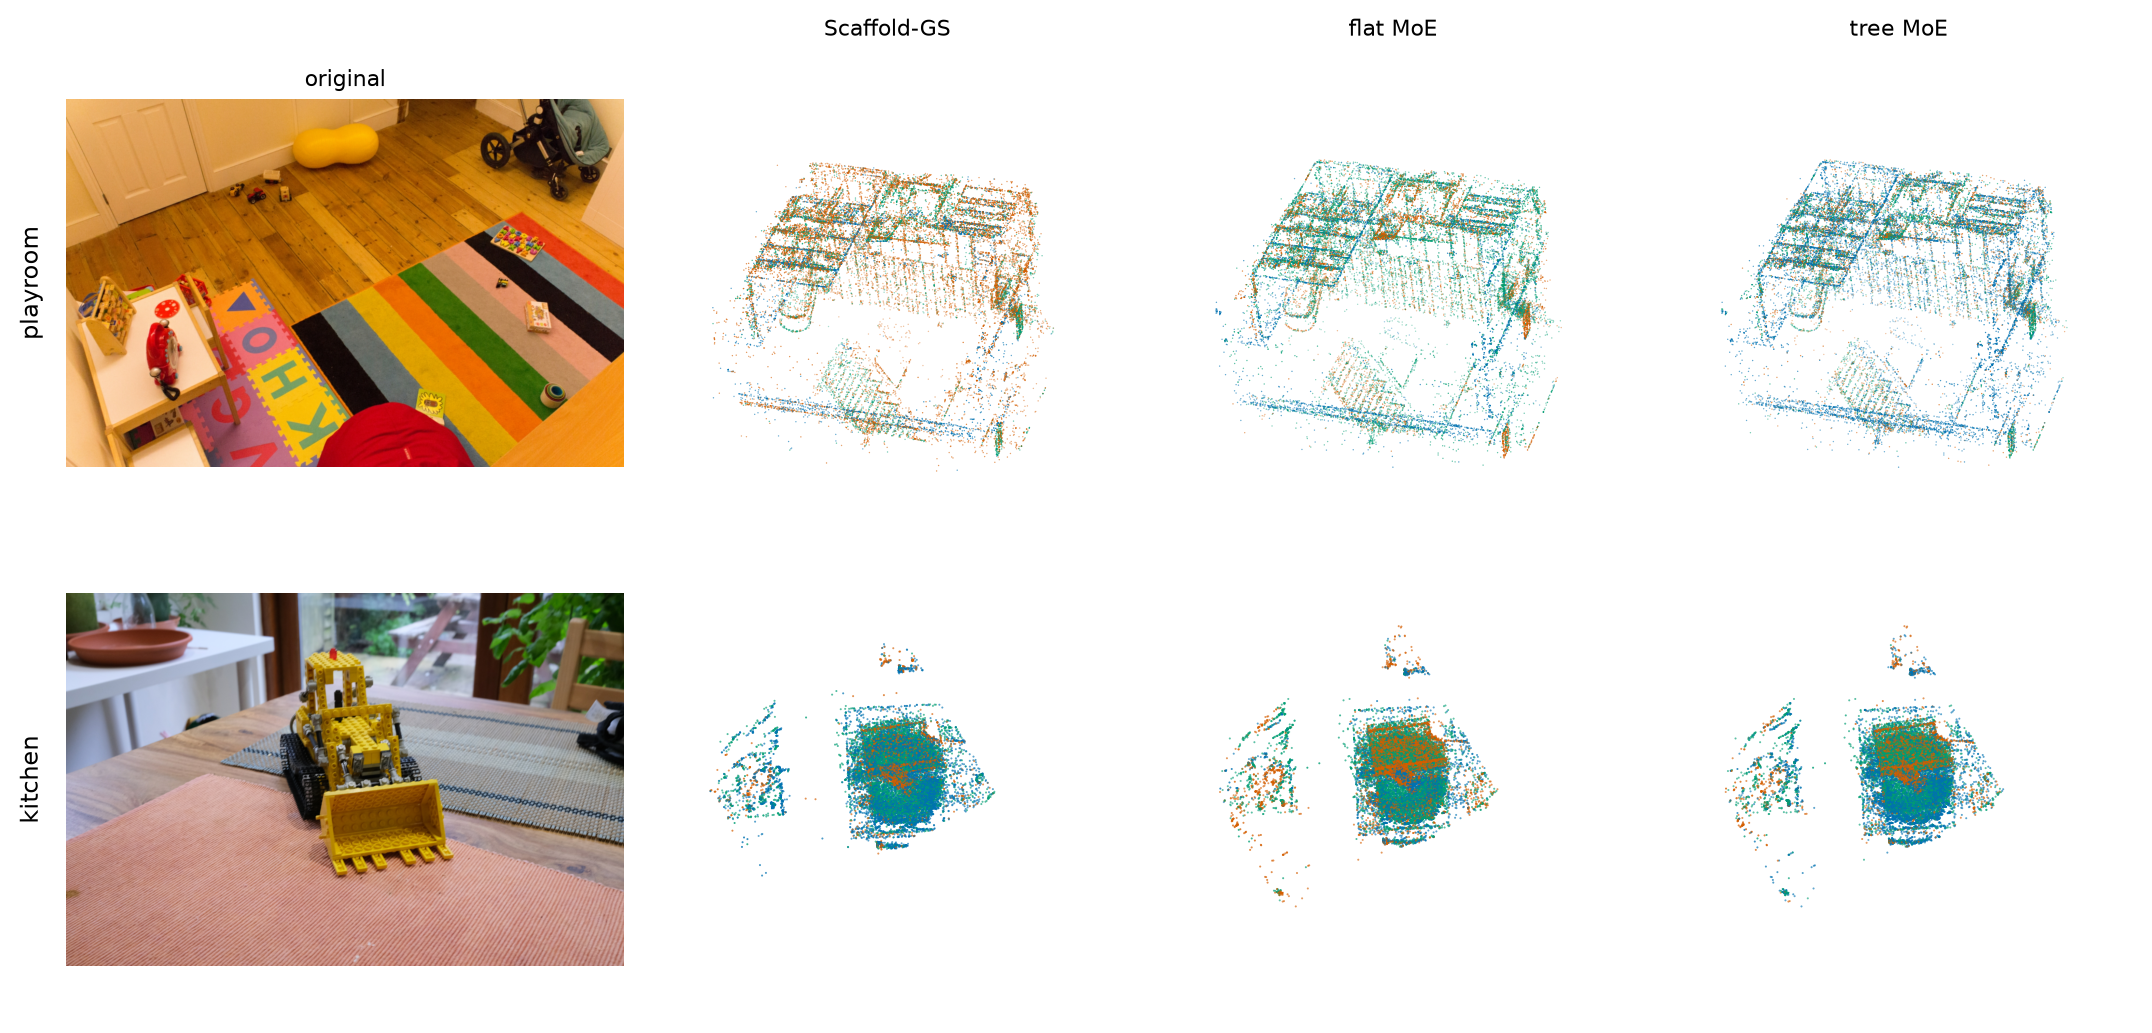
\includegraphics[width=\linewidth]{figures/anchor_feature_clustering.png}
  \caption{K-means ($K{=}3$) on stored anchor features $\mathbf{f}_i\in\mathbb{R}^{32}$.
  Color is the cluster index, not RGB and not the MoE expert.
  Left: photograph (context only).
  Right: $3$D anchors for Scaffold-GS, flat MoE, and Tree MoE on
  \texttt{playroom} (into the room) and \texttt{kitchen} (top-down; table at center).
  MoE training preserves the floor/object partition rather than mixing it.}
  \label{fig:clustering}
\end{figure*}
